To perform the statistical interpretation of the data, we use
the standard Higgs group combination tools~cite{lands}, \cite{combine}.
These tools require input cards describing the nuisance parameters
along with central and alternative shapes (histograms), which 
are required to be 1-dimensional.  Because the maximum likelihood
fit does not care how the bins are arranged, we ``unroll'' the 
2-dimensional histograms into the 1-dimensional format.

\begin{figure}[htp]
	\centering
	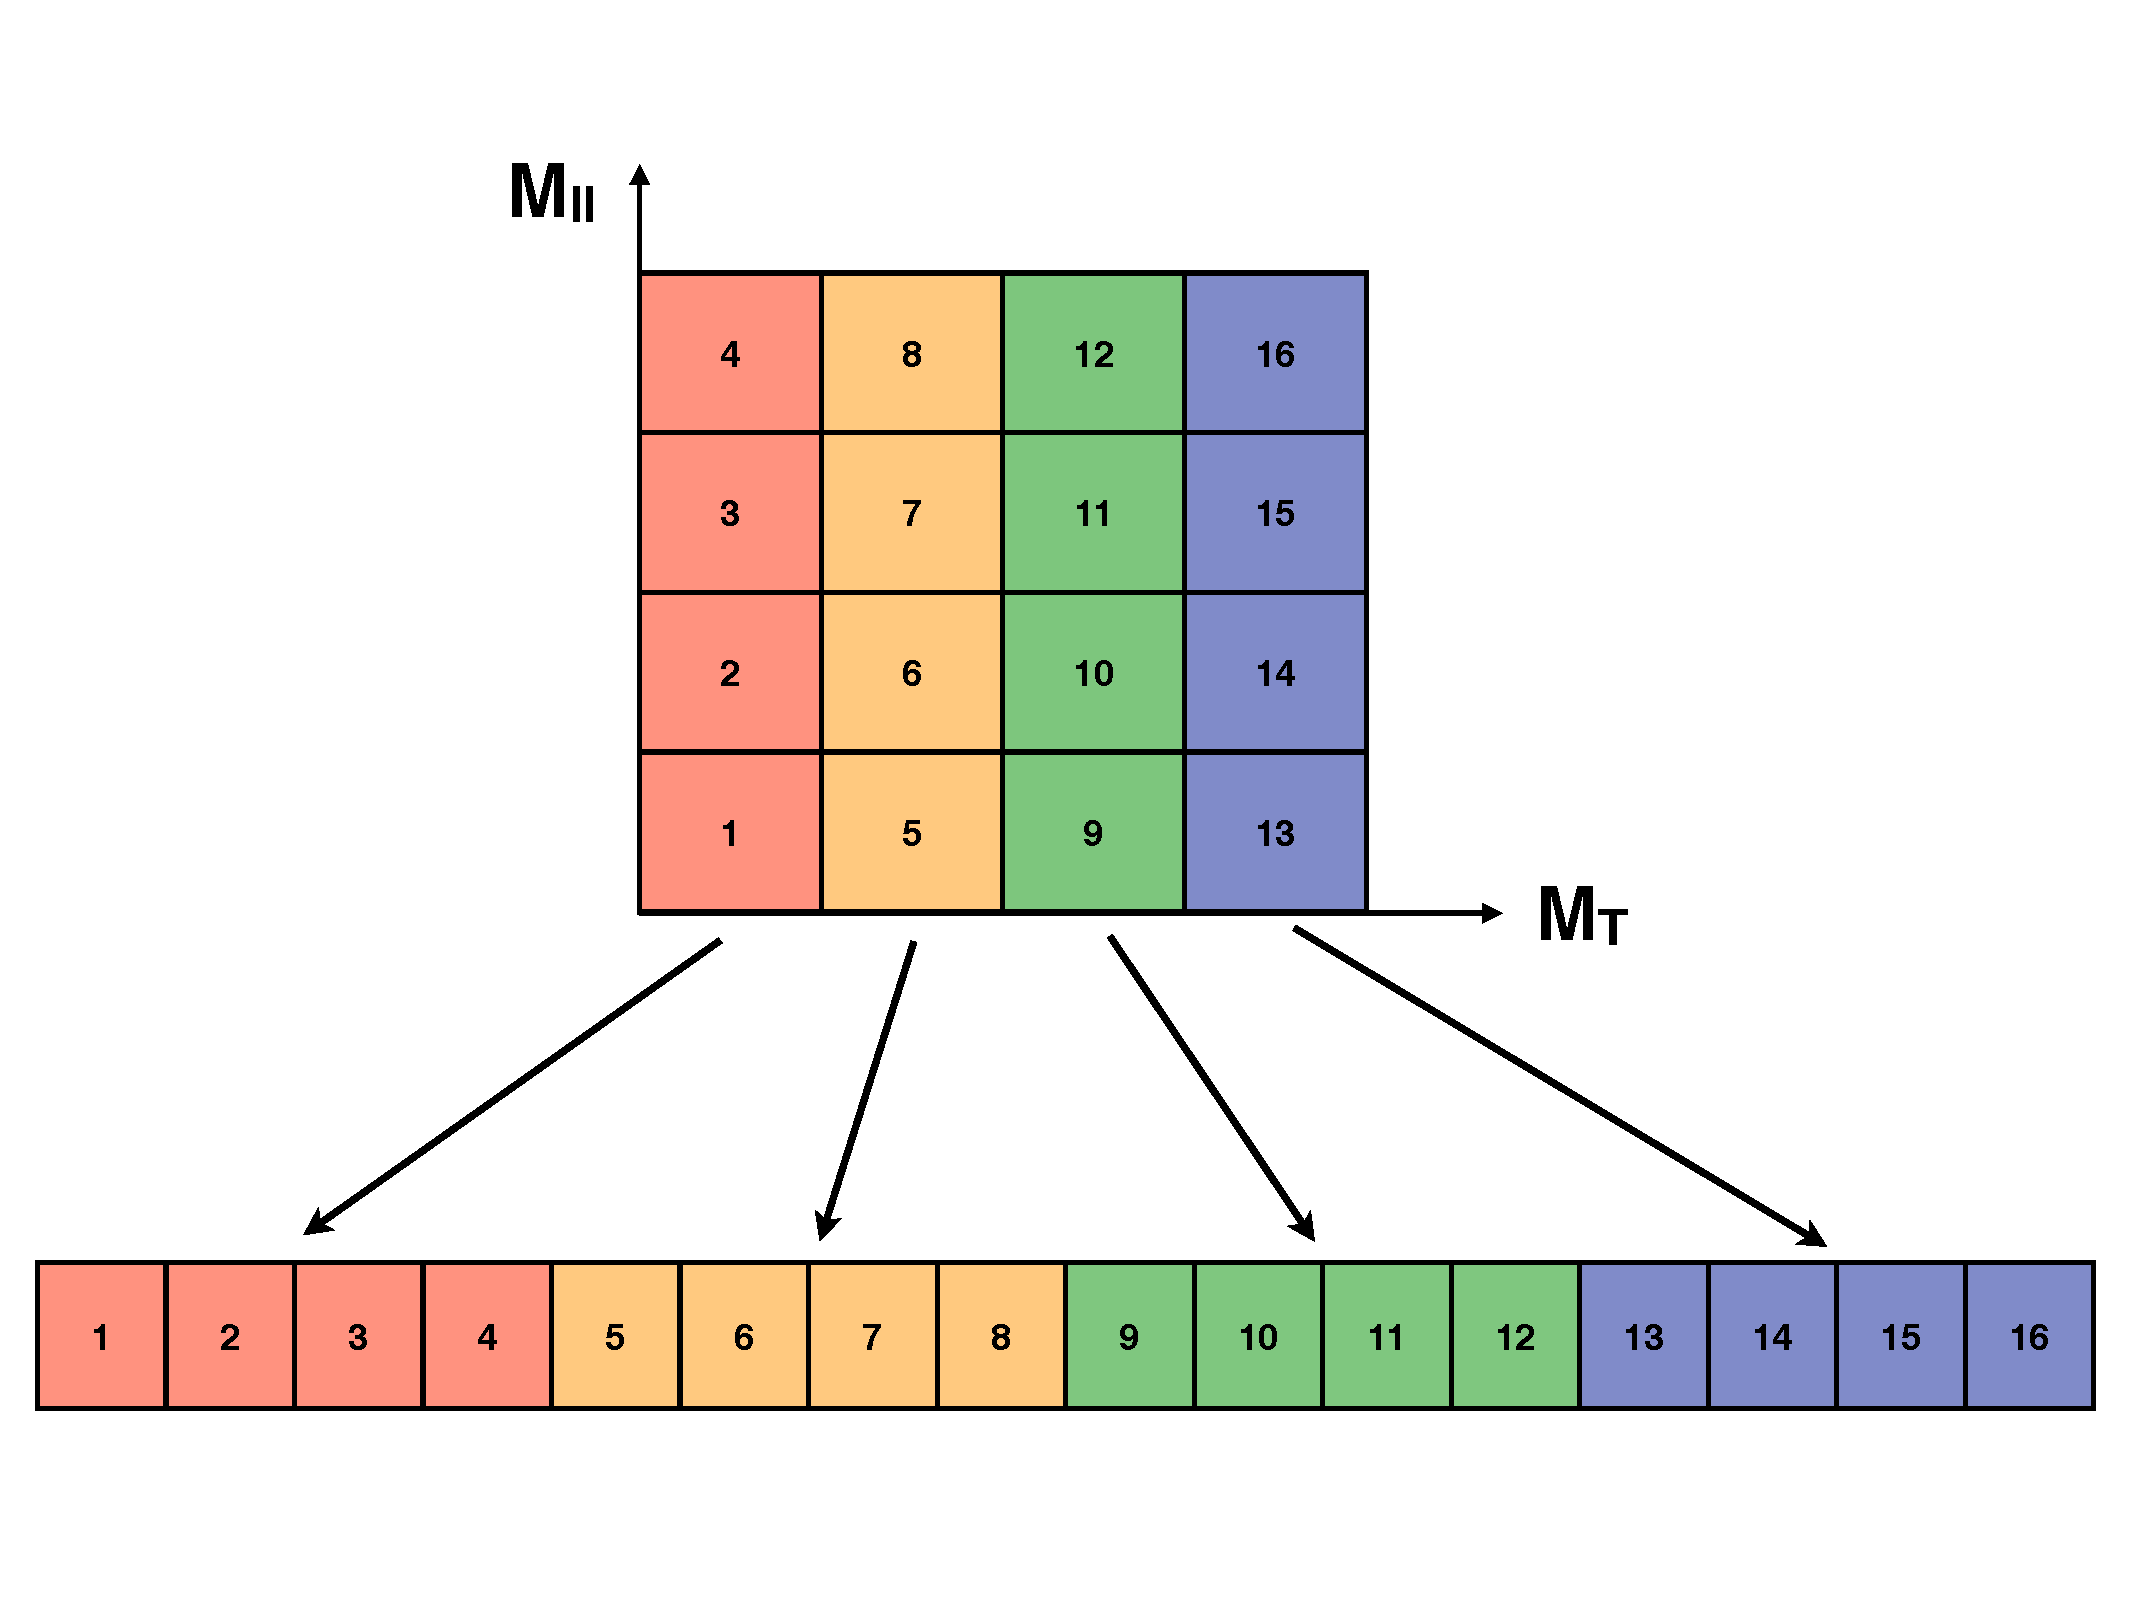
\includegraphics[width=0.8\textwidth]{figures/unrolling_schematic.pdf}
	\caption{ Schematic of how unrolling is done from 4x4 2D to 1D histogram. 
			  The numbers in the 2D and 1D histograms indicate the same bins.} 
  	\label{fig:unrolling_sch}
\end{figure}

Figure~\ref{fig:unrolling_sch} shows how the unrolling is done.
In the case of a 4x4 2D template, the first column in the 2D histogram 
becomes the 1st - 4th bins in the 1D histogram. The second column becomes 
5th - 8th bins in the 1D. Same thing goes until the last column.  
Figure~\ref{fig:unrolling_ex} shows an example of 2D template and
the corresponding unrolled template.

\begin{figure}[htp]
	\centering
	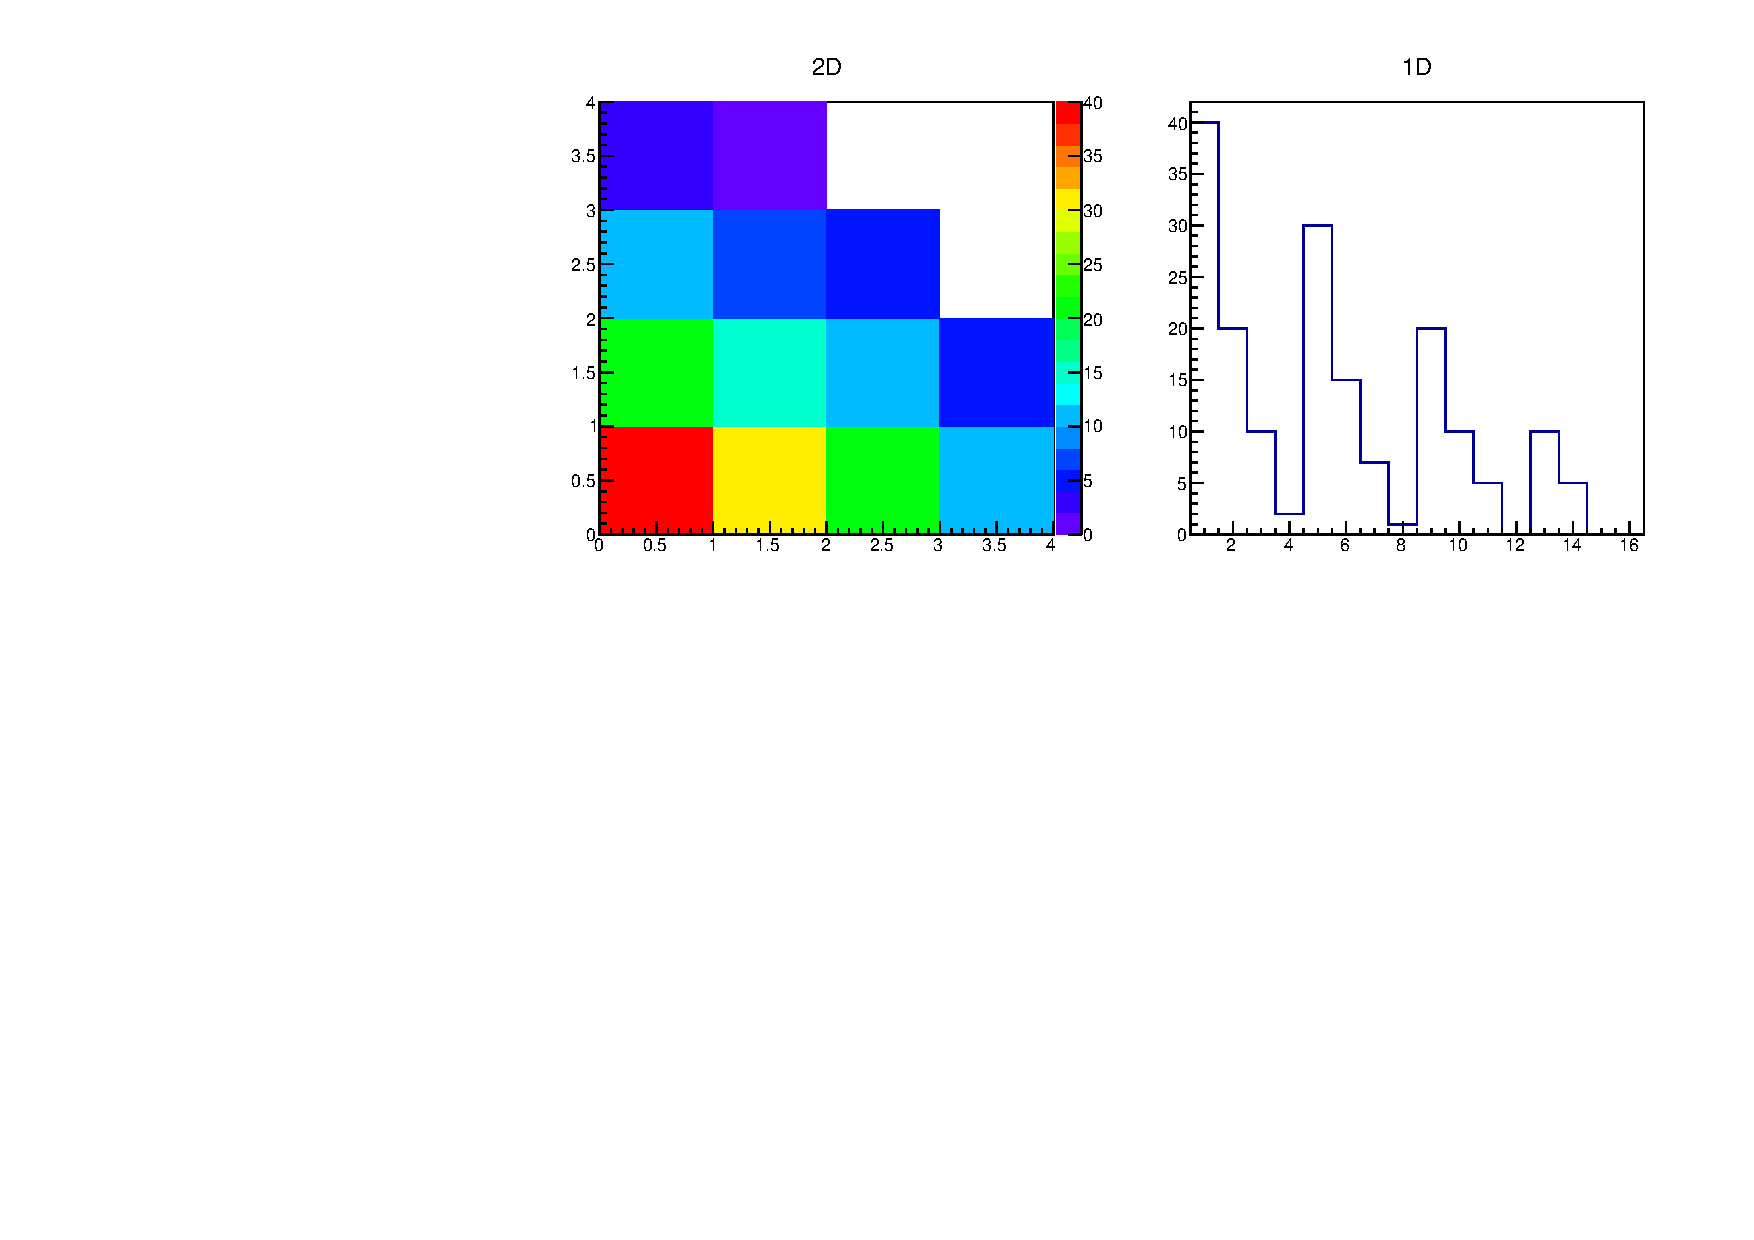
\includegraphics[width=0.8\textwidth]{figures/unrolling_example.pdf}
	\caption{ Example of how unrolling is done from 4x4 2D to 1D histogram.} 
  	\label{fig:unrolling_ex}
\end{figure}

